% Donor selection funnel (Section Donor Selection).
% Requires in the preamble: \usepackage{tikz}  \usepackage{xcolor}
\definecolor{funfill}{HTML}{6E8CAE}
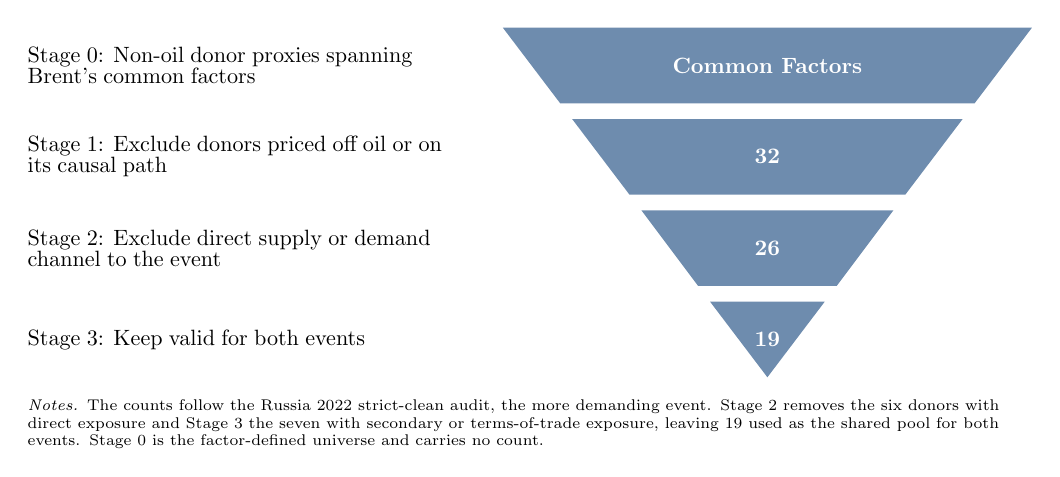
\begin{tikzpicture}[scale=0.8,transform shape,font=\footnotesize,
   bar/.style={anchor=west,align=left,text width=7.0cm,inner sep=0pt}]
  \def\cx{12}
  % inverted funnel, taper slope ~0.76; apex (cx,0.5), bands 1.2 tall with 0.25 gaps

  % ---- stage 0 : global categories (label only, the donor universe) ----
  \fill[funfill] (\cx-4.2,6.05) -- (\cx+4.2,6.05) -- (\cx+3.29,4.85) -- (\cx-3.29,4.85) -- cycle;
  \node[white,font=\normalsize\bfseries] at (\cx,5.45) {Common Factors};
  \node[bar] at (0.25,5.45) {{\normalsize Stage 0: Non-oil donor proxies spanning Brent's common factors}};

  % ---- stage 1 : 32 ----
  \fill[funfill] (\cx-3.1,4.6) -- (\cx+3.1,4.6) -- (\cx+2.19,3.4) -- (\cx-2.19,3.4) -- cycle;
  \node[white,font=\normalsize\bfseries] at (\cx,4.0) {32};
  \node[bar] at (0.25,4.0) {{\normalsize Stage 1: Exclude donors priced off oil or on its causal path}};

  % ---- stage 2 : 26 ----
  \fill[funfill] (\cx-2.0,3.15) -- (\cx+2.0,3.15) -- (\cx+1.1,1.95) -- (\cx-1.1,1.95) -- cycle;
  \node[white,font=\normalsize\bfseries] at (\cx,2.55) {26};
  \node[bar] at (0.25,2.55) {{\normalsize Stage 2: Exclude direct supply or demand channel to the event}};

  % ---- stage 3 : 19 (apex) ----
  \fill[funfill] (\cx-0.91,1.7) -- (\cx+0.91,1.7) -- (\cx,0.5) -- cycle;
  \node[white,font=\normalsize\bfseries] at (\cx,1.1) {19};
  \node[bar] at (0.25,1.1) {{\normalsize Stage 3: Keep valid for both events}};

  % ---- note ----
  \node[anchor=north west,align=left,text width=15.5cm,inner sep=0pt,font=\scriptsize]
     at (0.25,0.15) {\textit{Notes.} The counts follow the Russia 2022 strict-clean audit,
     the more demanding event. Stage 2 removes the six donors with direct exposure and Stage 3
     the seven with secondary or terms-of-trade exposure, leaving 19 used as the shared pool
     for both events. Stage 0 is the factor-defined universe and carries no count.};
\end{tikzpicture}
